\documentclass[]{article}


\usepackage[margin=1cm,includehead,landscape]{geometry}
\usepackage{fancyhdr}
\usepackage{multicol}
\usepackage{graphicx}
\pagestyle{fancy}
\usepackage{amsmath}
\usepackage{amssymb}
\usepackage{cancel}
\usepackage{float}
\usepackage{siunitx}
\usepackage{subfiles}
\usepackage{enumitem}
\usepackage{physics}
\usepackage[dvipsnames]{xcolor}

\fancyhead[L,RO]{}
\fancyfoot[L,RO]{}

\sisetup{range-phrase=...}

\newcommand{\cdelay}{\textcolor{RoyalBlue!75!Black}{\mathbf{cd}}}
\newcommand{\pdelay}{\textcolor{OrangeRed!75!Black}{\mathbf{pd}}}
\newcommand{\cdel}{\textcolor{RoyalBlue!75!Black}{\mathbf{c}}}
\newcommand{\pdel}{\textcolor{OrangeRed!75!Black}{\mathbf{p}}}

\begin{document}
\fancyhead[C]{PCB}
\subfile{pcb}
\pagebreak
\fancyhead[CO]{Analogique}
\subfile{opamp}
\pagebreak
\subfile{opamp1}
\pagebreak
\subfile{opamp2}
\pagebreak
\subfile{opamp3}
\pagebreak
\subfile{adc}
\pagebreak

\fancyhead[CO]{Numérique}
\subfile{timing}
\pagebreak
\subfile{circuits}
\pagebreak
\begin{center}
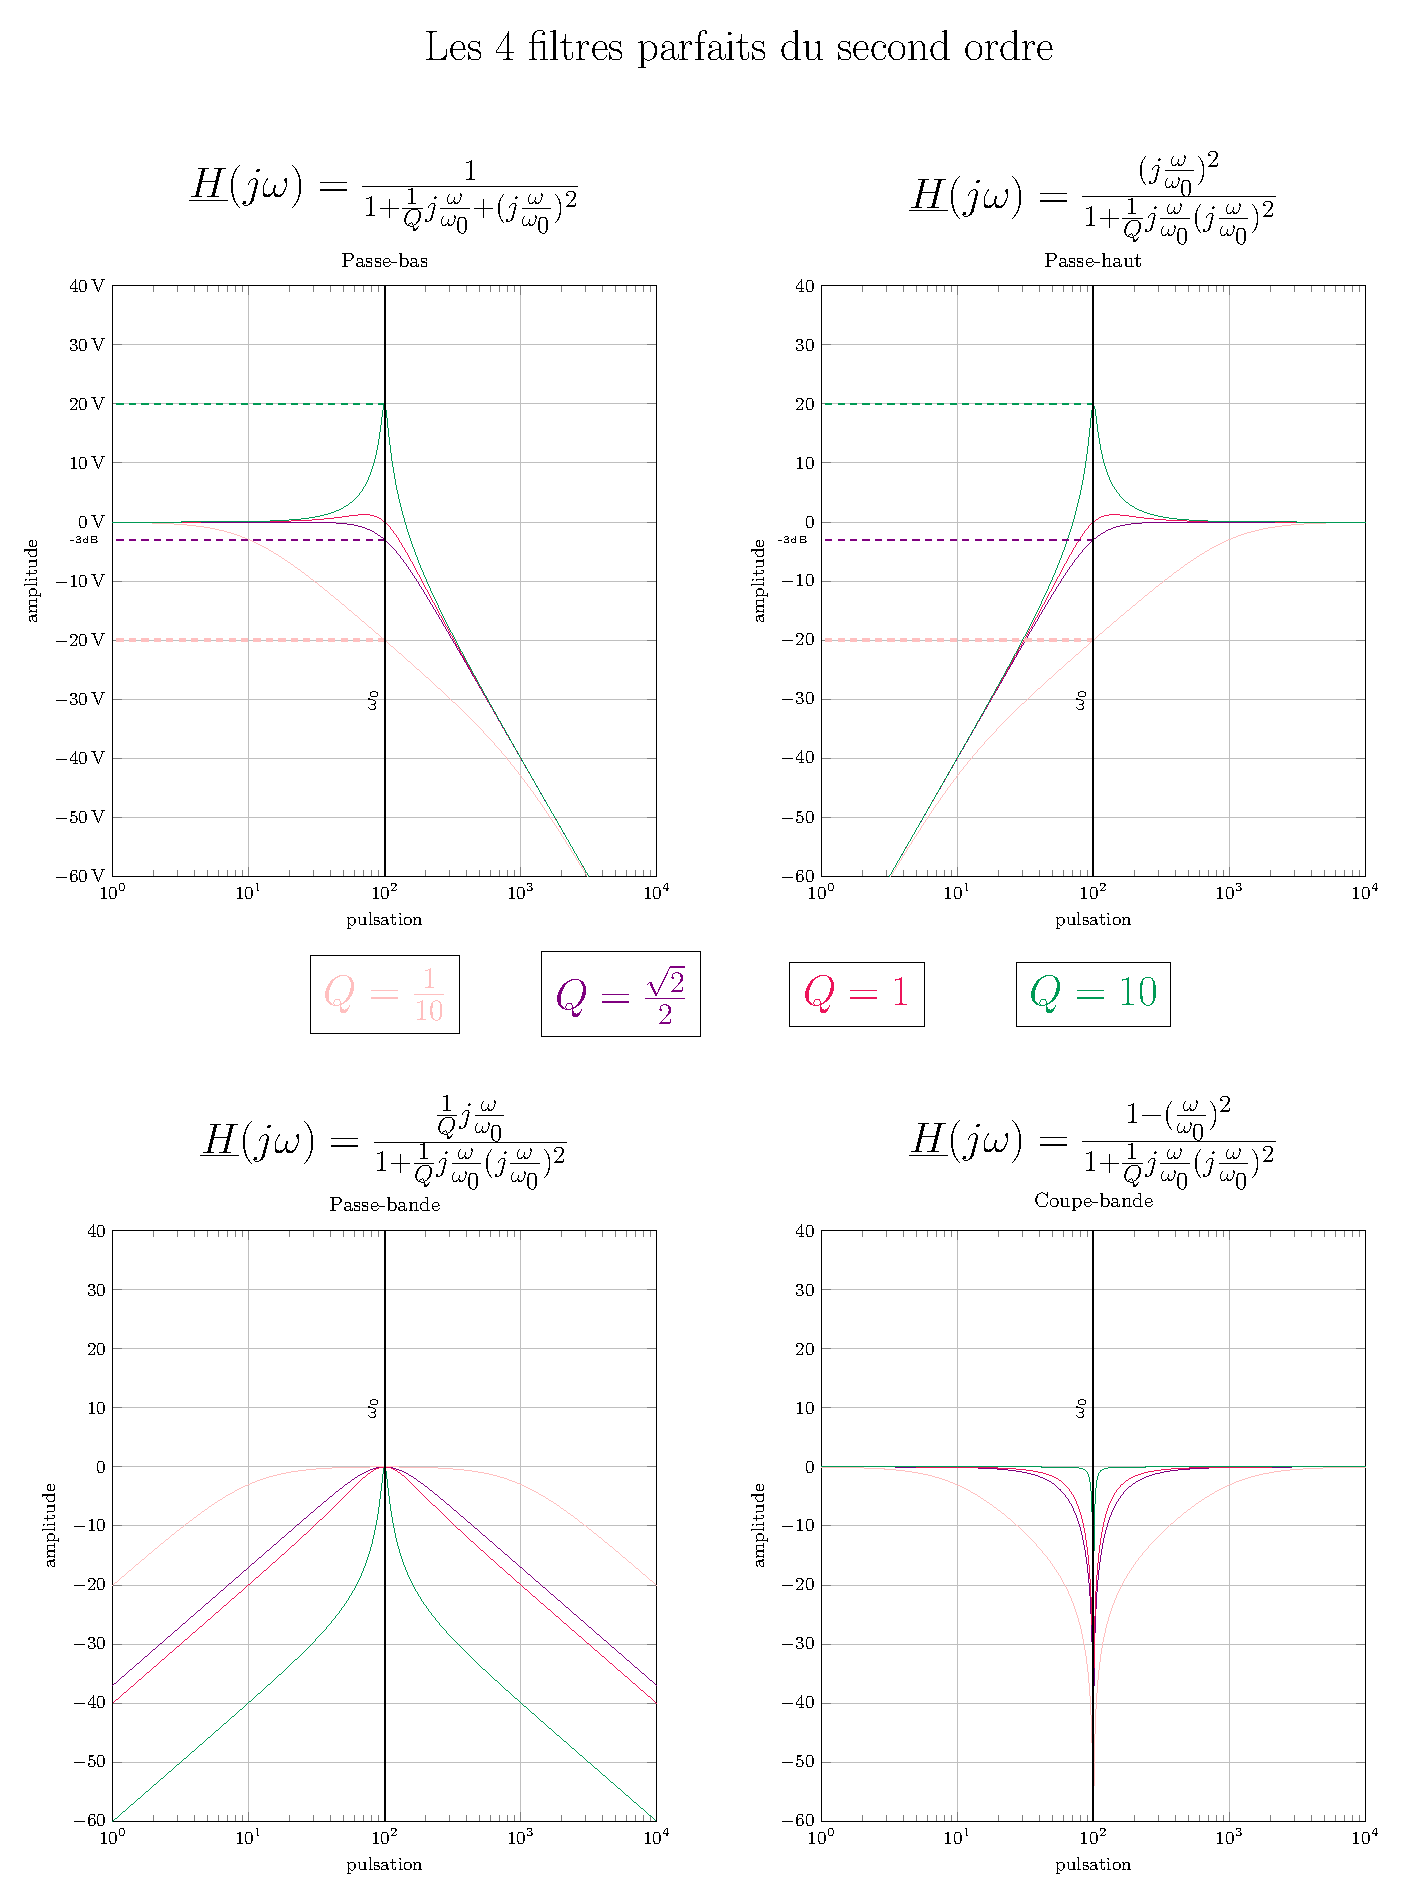
\includegraphics[height=\textheight]{Bode2.pdf}
\end{center}



\end{document}


